\documentclass[11pt]{article}
\usepackage{geometry}                % See geometry.pdf to learn the layout options. There are lots.
\geometry{letterpaper}                   % ... or a4paper or a5paper or ... 
%\geometry{landscape}                % Activate for for rotated page geometry
%\usepackage[parfill]{parskip}    % Activate to begin paragraphs with an empty line rather than an indent
\usepackage{graphicx}
\usepackage{amssymb}
\usepackage{amsmath}
\usepackage{epstopdf}
\usepackage{hyperref}
\DeclareGraphicsRule{.tif}{png}{.png}{`convert #1 `dirname #1`/`basename #1 .tif`.png}


\graphicspath{
{/Users/Andy/Cruises_Research/Analysis/Andy_Pickering/eq14_patch_gamma/figures/}
{/Users/Andy/Cruises_Research/Analysis/Andy_Pickering/eq14_patch_gamma/figures/chi_eps_profiles_diffNprof_profavgs/zsm10m_fmax7Hz_respcorr0_fc_99hz_gamma20_nfft_128_screen_chi_1/}
}

\title{Estimating $\epsilon$ from fast thermistors $\chi$pod ?}
\author{Andy Pickering}
%\date{}                                           % Activate to display a given date or no date



\begin{document}
\maketitle

\tableofcontents
\newpage



%~~~~~~~~~~~~~~~~~~~~~~~~~~~~~~~~~~~~~~~~
\section{Abstract}
%~~~~~~~~~~~~~~~~~~~~~~~~~~~~~~~~~~~~~~~~

The acquisition of turbulence data from shipboard CTD profiles is attractive, as it has the potential to significantly increase the amount of deep-ocean mixing observations globally.  While data from shear-probes are easily contaminated by motion of the instrument platform, the measurement of temperature gradient is relatively insensitive to vehicle vibration, making it possible to measure temperature gradient from a shipboard CTD rosette.  The purpose of this note is to investigate the error and bias in estimating the rate of dissipation of temperature variance $\chi$ from fast thermistors mounted on traditional CTD casts.  The most significant source of error is associated with the fact that fast-response FP07 thermistors resolve only a fraction of the temperature gradient variance at the fallspeed of typical CTD casts.  Assumptions must be made about the wavenumber extent of the temperature gradient spectrum, which scales with the rate of dissipation of turbulent kinetic energy, a quantity that is not directly measured.  Here we utilize observations from a microstructure profiler with shear probes to demonstrate the validity of our method of estimating $\chi$ from thermistor data, and to assess uncertainty and bias. This supports the utility of the measurement as part of the global repeat hydrography program (GO-SHIP) cruises, during which this type of data has been acquired during the past few years.

%We then apply this methodology to temperature gradient profiles obtained from $\chi$pods mounted on a CTD (the CTD-$\chi$pod), and compare these to microstructure profiles obtained almost synoptically at the equator.  CTD-$\chi$pod estimates of $\chi$ compare favorably to the shear-probe microstructure measurements and demonstrate that the $\chi$pod method is not significantly biased


%~~~~~~~~~~~~~~~~~~~~~~~~~~~~~~~~~~~~~~~~
\section{Introduction}
%~~~~~~~~~~~~~~~~~~~~~~~~~~~~~~~~~~~~~~~~

The main points are that gamma (computed the way we do) is not equal to 0.2, but when you compute epsilon from chi, if is appropriate to use gamma=0.2 to get the answer right, because, for the epsilons that matter (the ones that dominate the mean), gamma=0.2 gives you the correct answer.

\begin{itemize}

\item This document is an attempt to provide an overview/summary of what i've found in my $\chi$pod analysis so far. 

\item The motivation/goal for all this work is to show if /how well the CTD-$\chi$pod method works for estimating $\chi$,$\epsilon$, $K_T$, etc from fast temperature (thermistor) profiles. The idea is to deploy $\chi$pods on regular CTD casts on WOCE/CLIVAR cruises etc. to making mixing measurements.

\item Before dealing with all the issues with the CTD deployments (depth loops, entrained water, rosette-induced turbulence etc.), I wanted to verify that the method itself worked w/out these complications. 

\item The Chameleon microstructure profiler has both thermistor and shear probes, so this seemed like an ideal way to test the method. I would apply the $\chi$pod method to the chameleon thermistor data only ($\chi_{\chi},\epsilon_{\chi}$), and compare to the `true' results computed using the shear probes ($\chi$,$\epsilon$).

\item I found that the estimates of $\chi$ agreed well, but $\epsilon_{\chi}$ was biased low compared to $\epsilon$ (Figure \ref{chi_overview},\ref{eps_overview},\ref{chamVschi}).

\item The $\chi$pod method requires assuming a mixing efficiency, and uses the normal assumption that $\gamma=0.2$. I computed gamma from the chameleon data (formula) and found that it was about an order of magnitude smaller than 0.2; hence the low epsilon estimates?
\item The comparison of $\epsilon_{\chi}$ to $\epsilon$ seems to improve with increased averaging (of either multiple profiles or larger depth ranges). 

\end{itemize}




\clearpage
%~~~~~~~~~~~~~~~~~~~~~~~~~~~~~~~~~~~~~~~~
\section{Data and Processing}
%~~~~~~~~~~~~~~~~~~~~~~~~~~~~~~~~~~~~~~~~

\begin{itemize}

\item Data are from Chameleon profiles near the equator during the `EQ14' experiment.

\item Sally shared w/ me Chameleon data that she and Jim processed. I ended up re-processing it using a smaller fmax (7Hz) because it looked like the thermistor spectra rolled off much lower than the assumed 32Hz.

\item \verb+ComputeChi_Chameleon_Eq14.m+ : Applies $\chi$pod method to Chameleon profiles from EQ14.

\item \verb+Make_Overview_Plots.m+ Makes almost all the figures in this document.

\item The noise floor of Chamleon $\epsilon$ was determined to be $log_{10}[\epsilon]=-8.5$. Values below this threshold were discarded. $\chi$pod values below this threshold were also discarded, in order to make a valid comparison. An upper limit of $log_{10}[\epsilon]=-5$ (determined by Jim?) was also applied.

\end{itemize}




\clearpage
%~~~~~~~~~~~~~~~~~~~~~~~~~~~~~~~~~~~~~~~~
\section{Results}
%~~~~~~~~~~~~~~~~~~~~~~~~~~~~~~~~~~~~~~~~


\subsection{Overview}

% misc_Appr14.m
\begin{figure}[htbp]
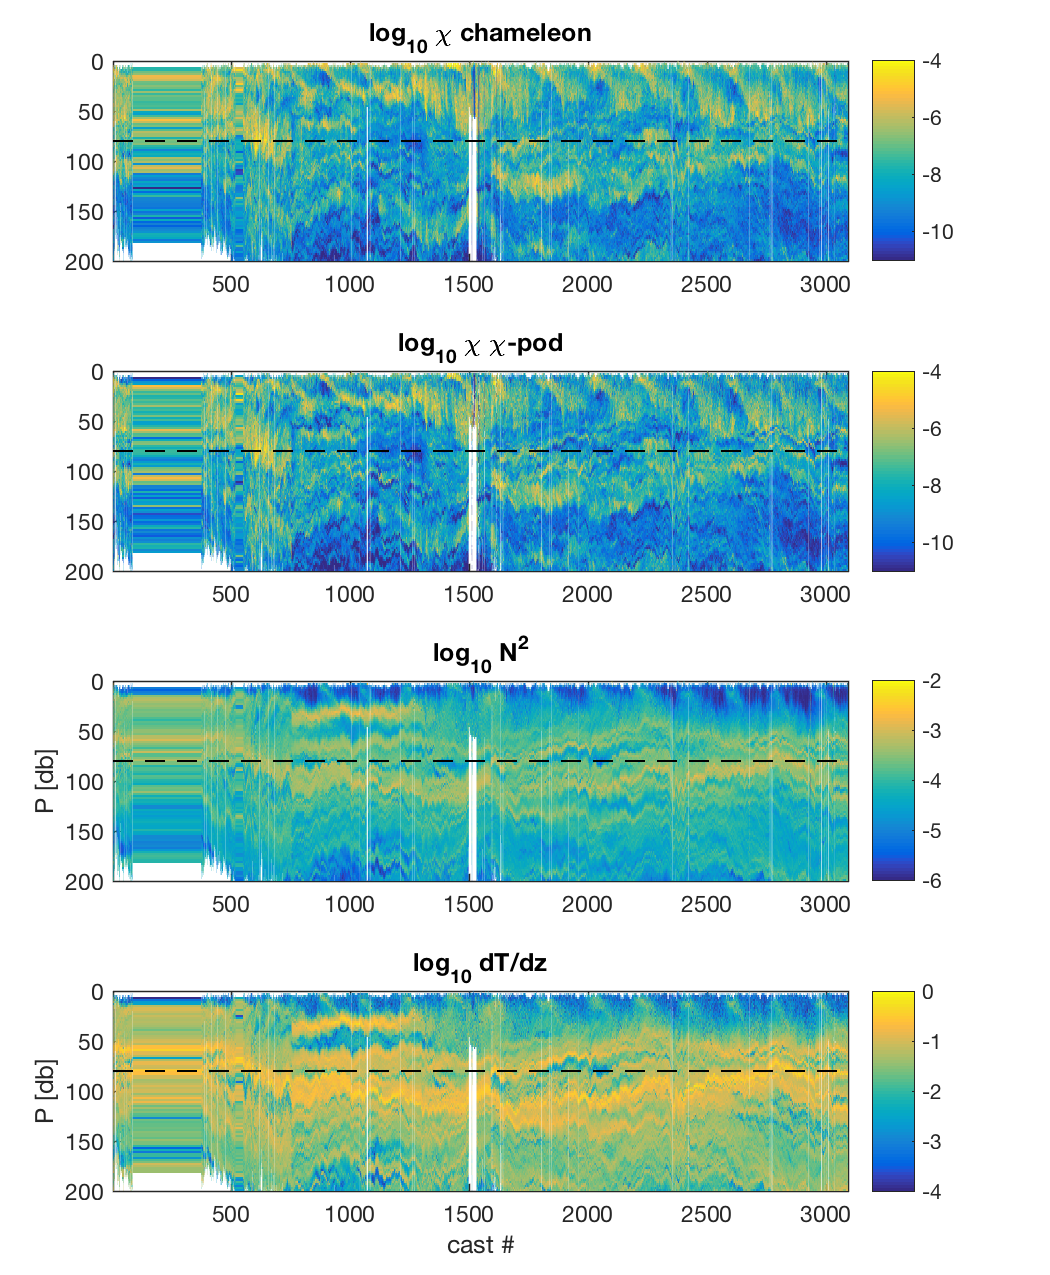
\includegraphics[scale=0.8]{eq14_Pcolor_BothChi_N2_Tz_zsmooth_10_2mbin_screen_chi_1.png}
\caption{Comparison of $\chi$ from chameleon method and chi-pod method, for EQ14 chameleon profiles. Each profile was averaged in 2m bins.  Horizontal line at 80m shows region excluded in further analysis because it contains near-surface convection.}
\label{chi_overview}
\end{figure}

\begin{figure}[htbp]
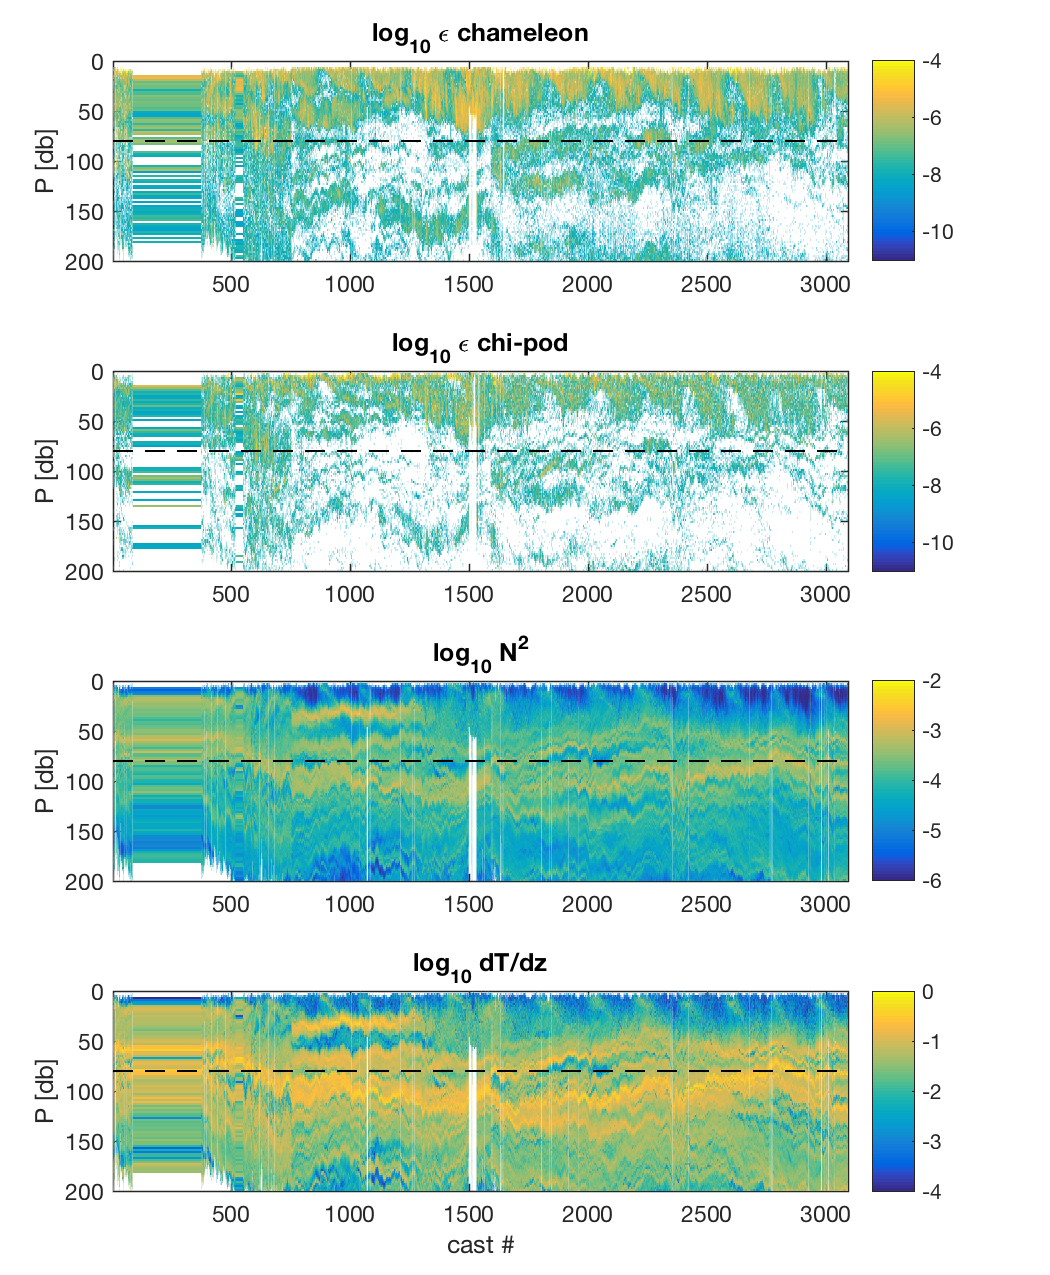
\includegraphics[scale=0.8]{eq14_Pcolor_BothEps_N2_Tz_zsmooth_10_2mbin_screen_chi_1.png}
\caption{Comparison of $\epsilon$ from chameleon method and chi-pod method, for EQ14 chameleon profiles. Each profile was averaged in 2m bins.  Values of $\epsilon$ below chameleon noise floor ($log_{10}[\epsilon]=-8.5$) have been nan'd out. Horizontal line at 80m shows region excluded in further analysis because it contains near-surface convection.}
\label{eps_overview}
\end{figure}





%    \clearpage
%    %~~~~~~~~~~~~~~~~~~~~~~~~~~~~~~~~~~~~~~~~
%    \subsection{Comparing individual estimates of $\epsilon$}
%    %~~~~~~~~~~~~~~~~~~~~~~~~~~~~~~~~~~~~~~~~
%    
%    \begin{figure}[htbp]
%    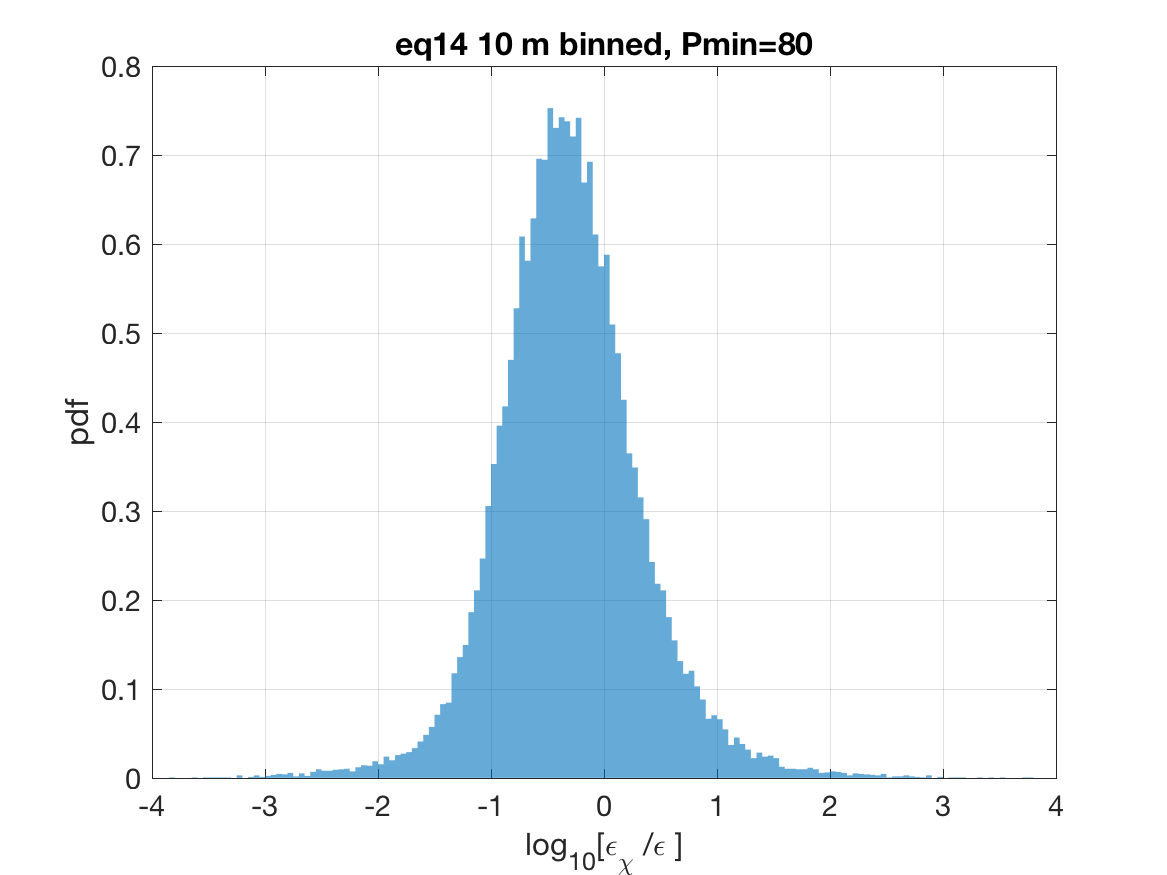
\includegraphics[scale=0.8]{eq14_10mbinned_eps_ratios_Pmin80_screen_chi_1.png}
%    \caption{EQ14: Histogram of the ratio of $\epsilon$ estimates from $\chi$pod method to the chameleon values, for $\chi$pod method applied to 1m binned profiles, and applied to just patches. Estimates for each profile were averaged in 10m depth bins. Vertical line shows mean of $log_{10}[\epsilon_{\chi}/\epsilon]$.}
%    \label{epsrathist_eq14}
%    \end{figure}





\clearpage
%~~~~~~~~~~~~~~~~~~~~~~~~~~~~~~~~~~~~~~~~
\subsection{Normalized eps vs chi plots}
%~~~~~~~~~~~~~~~~~~~~~~~~~~~~~~~~~~~~~~~~

Assuming that
\begin{equation}
\gamma=\frac{N^2 \chi}{2\epsilon<T_z>^2}
\end{equation}
, plotting [$\chi/t_{z}^{2}$] vs [$\epsilon/N\^2$] should follow a straight line with slope equal to $2\gamma$.


\begin{figure}[htbp]
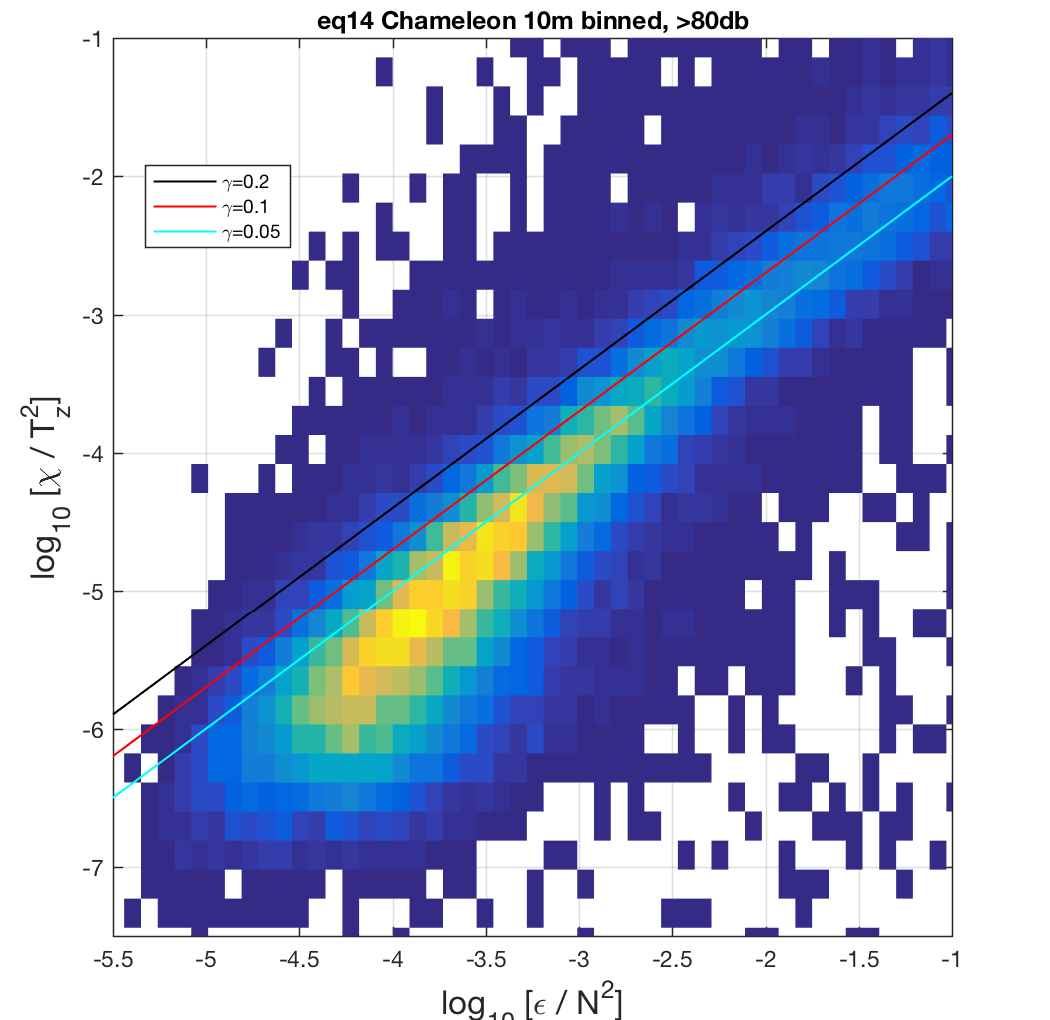
\includegraphics[scale=0.8]{eq14_10mbinned_eps_vs_chi_normalized_Pmin_80.png}
\caption{EQ14: 10m binned  chameleon $\epsilon/N\^2$ vs $\chi/t_{z}^{2}$ for *below 80db*. Lines show different values of $\gamma$. Values of $\epsilon$ below noise floor ($log_{10}\epsilon<-8.5$) are discarded also.}
\label{}
\end{figure}





\clearpage
%~~~~~~~~~~~~~~~~~~~~~~~~~~~~~~~~~~~~~~~~
\subsection{Averaging many profiles of $\epsilon$}
%~~~~~~~~~~~~~~~~~~~~~~~~~~~~~~~~~~~~~~~~

Figure \ref{prof_avg_ex} shows one example. A folder with many profiles is located at:
\url{https://github.com/OceanMixingGroup/Analysis/tree/master/Andy_Pickering/eq14_patch_gamma/figures/chi_eps_profiles_40profavgs}. %In general, it seems that averaging profiles does not change the comparsion much; $\epsilon_{\chi}$ is still biased low.

\begin{figure}[htbp]
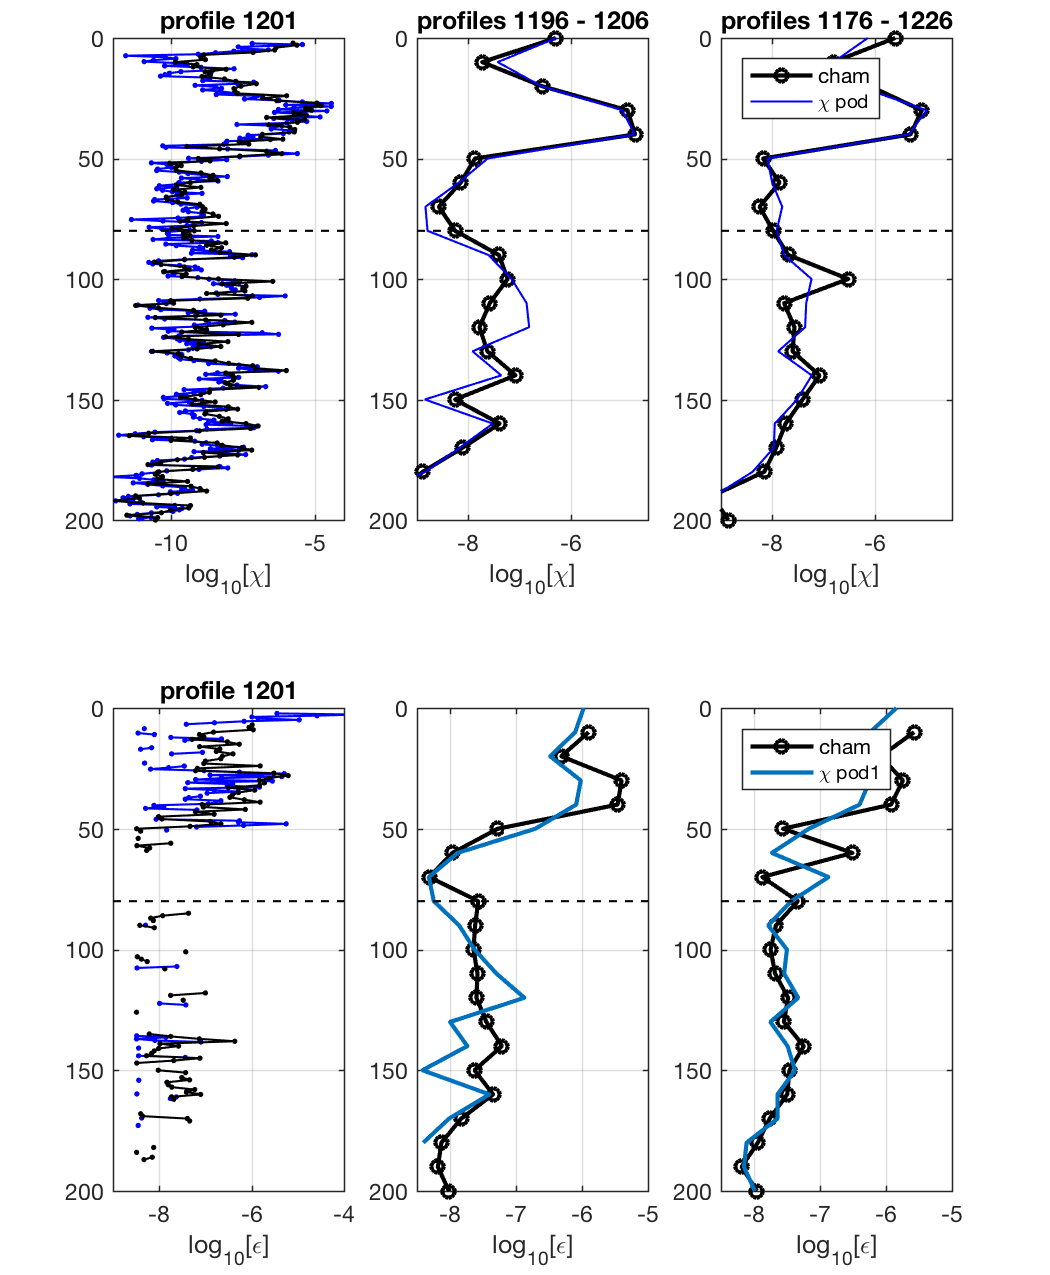
\includegraphics[scale=0.8]{eq14_profile_1201_eps_profiles_compare.png}
\caption{Example of averaging multiple profiles together. Left panels show a single profile from chamleeon and chi-pod method. Right panels show average of $+/-$ 40 profiles, averaged in 10m depth bins.}
\label{prof_avg_ex}
\end{figure}


\begin{figure}[htbp]
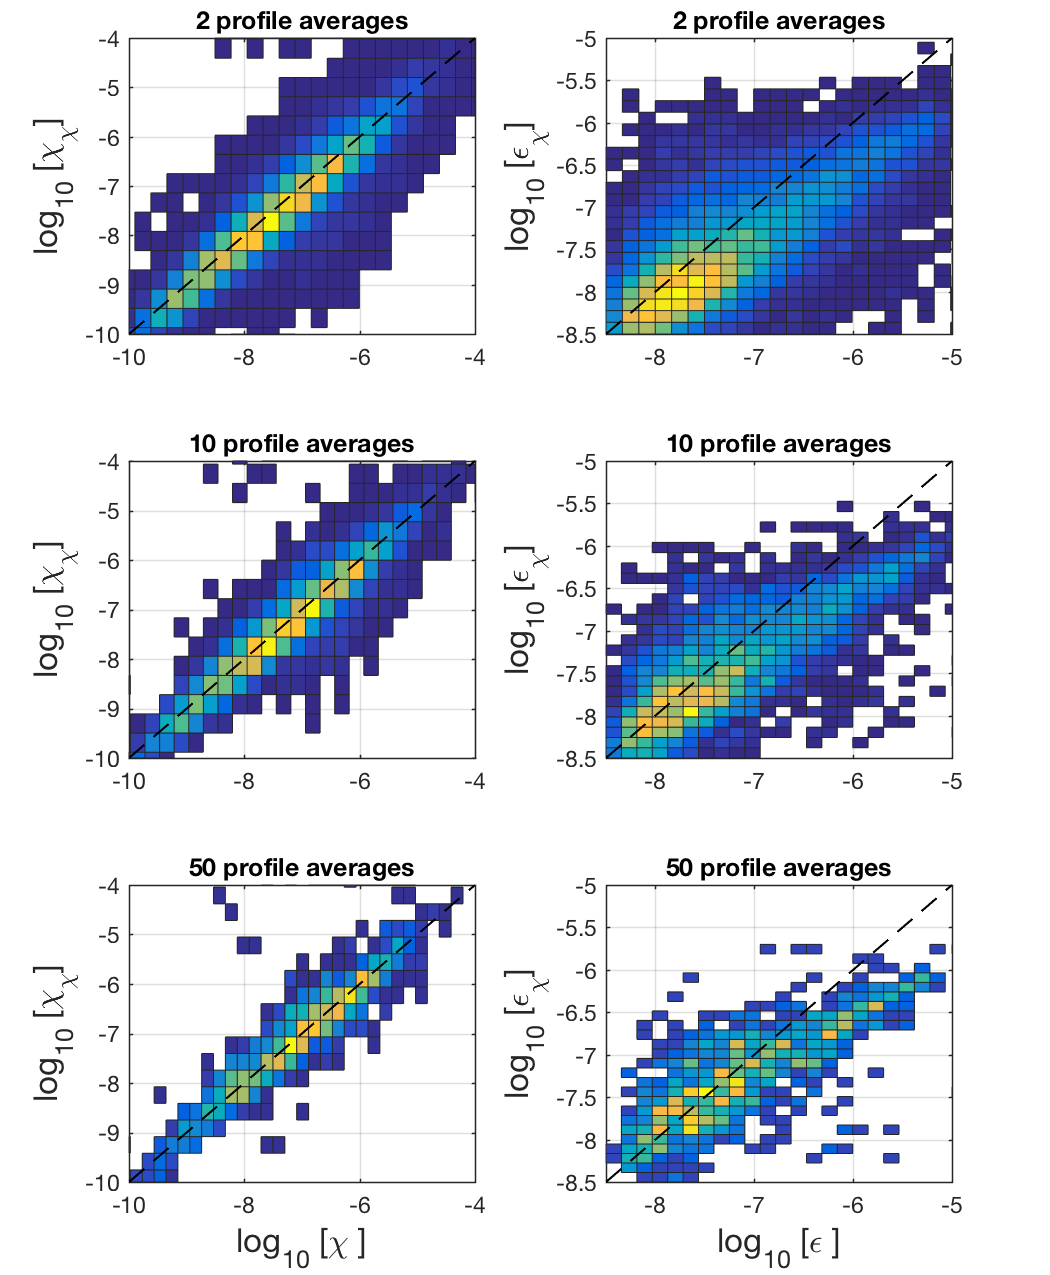
\includegraphics[scale=0.8]{eq14_chiVscham_chiANDeps_diff_prof_avg_screen_chi_1.png}
\caption{2D Histograms of $\chi_{chi}$ vs $\chi$ (left) and $\epsilon_{\chi}$ vs $\epsilon$ (right) for different numbers of profiles averaged.}
\label{}
\end{figure}


\begin{figure}[htbp]
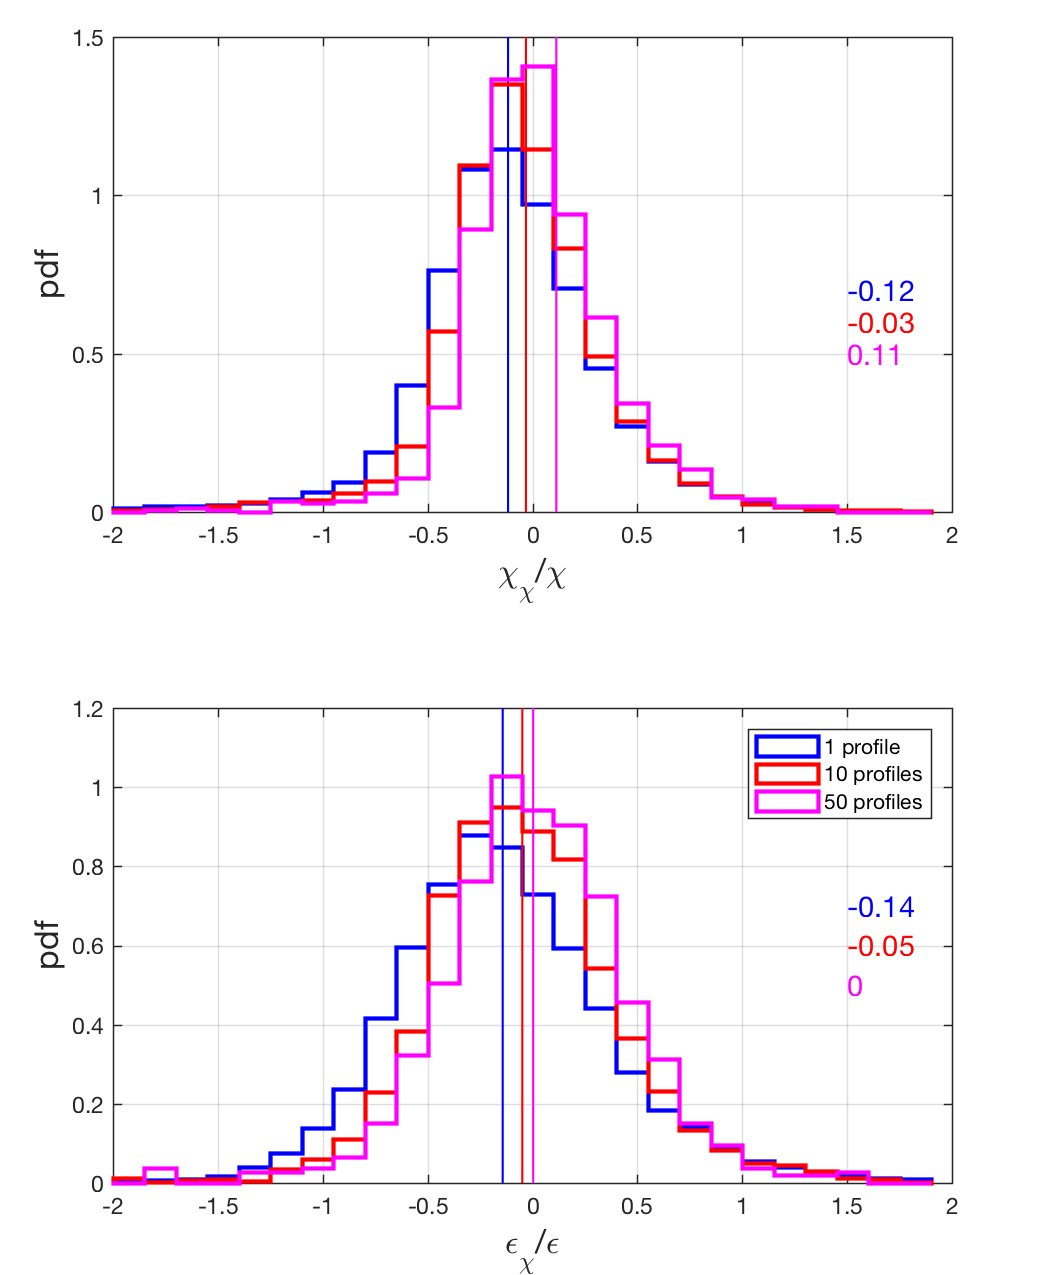
\includegraphics[scale=0.8]{eq14_eps_ratio_hist_diff_prof_avg.png}
\caption{(log10) Ratio of $\epsilon_{\chi}/\epsilon$ for different numbers of profiles averaged. Consecutive chunks of N profiles were averaged, and then (normalized) histogram of the ratios was plotted. Vertical lines are mean of $log_{10}[\epsilon_{\chi}/\epsilon]$ for each distribution. }
\label{}
\end{figure}











\clearpage
%~~~~~~~~~~~~~~~~~~~~~~~~~~~~~~~~~~~~~~~~
\section{Summary}
%~~~~~~~~~~~~~~~~~~~~~~~~~~~~~~~~~~~~~~~~

\begin{itemize}

\item Inidivudal (and 10m binned) $\chi$pod estimates of $\epsilon_{\chi}$ are biased low compared to Chameleon $\epsilon$.

\item This appears to be because $\gamma$ computed from the Chameleon data is lower than the assumed 0.2

\item $\gamma$ computed from averaged (across profiles) $N^2$, $T_z$, $\chi$, and $\epsilon$ is closer to 0.2

\item Averaging many $\epsilon$ profiles reduces the bias (if we use same noise floor for $\epsilon$ as Chameleon).

\item Increased depth-averaging also reduces bias.

\end{itemize}




\end{document}  


